% !TEX encoding = UTF-8 Unicode

% Geoscientific Model Development (gmd)
\documentclass[gmd, manuscript]{copernicus}

% packages
\usepackage{tabu}
\usepackage{booktabs}
\usepackage{graphicx}
\usepackage[export]{adjustbox}
\usepackage[utf8]{inputenc}
\usepackage{listings}
\usepackage[percent]{overpic}

\begin{document}

%\title{\lowercase{r.sim.terrain 1.0}: a dynamic landscape evolution model} 
\title{\lowercase{r.sim.terrain 1.0}: a landscape evolution model with dynamic hydrology} 

\Author[1]{Brendan Alexander}{Harmon}
\Author[2,3]{Helena}{Mitasova}
\Author[2,3]{Anna}{Petrasova}
\Author[2,3]{Vaclav}{Petras}

\affil[1]{Robert Reich School of Landscape Architecture, Louisiana State University, Baton Rouge, Louisiana, USA}
\affil[2]{Center for Geospatial Analytics, North Carolina State University, Raleigh, North Carolina, USA}
\affil[3]{Department of Marine, Earth, and Atmospheric Sciences, North Carolina State University, Raleigh, North Carolina, USA}

%\runningtitle{\lowercase{r.sim.terrain 1.0}: a dynamic landscape evolution model}
\runningtitle{\lowercase{r.sim.terrain 1.0}: a landscape evolution model with dynamic hydrology} 

\runningauthor{Brendan Harmon}

\correspondence{Brendan Harmon (baharmon@lsu.edu)}

\received{}
\pubdiscuss{}
\revised{}
\accepted{}
\published{}

\firstpage{1}

\maketitle

\begin{abstract}
While there are numerical landscape evolution models
that simulate how steady state flows of water and sediment
reshape topography over long periods of time, 
r.sim.terrain is the first to 
simulate short-term topographic change 
for both steady state and dynamic flow regimes
across a range of spatial scales.
This free and open source, 
GIS-based topographic evolution model
uses empirical models for soil erosion
at watershed to regional scales 
and a physics-based model
for shallow overland water flow and soil erosion 
at subwatershed scales
to compute short-term topographic change. 
This model uses either a steady state or dynamic representation of overland flow
to simulate how overland sediment mass flows reshape topography
for a range of hydrologic soil erosion regimes
based on topographic, land cover, soil, and rainfall parameters. 
As demonstrated by a case study 
for Patterson Branch subwatershed
on the Fort Bragg military installation in North Carolina,
r.sim.terrain can realistically simulate the development of 
fine-scale morphological features including 
ephemeral gullies, rills, and hillslopes.
Applications include land management, erosion control,
landscape planning, and landscape restoration. 
\end{abstract}

\copyrightstatement{...}

% --------- INTRO FIGURE ---------

\begin{figure}%[H]
\center
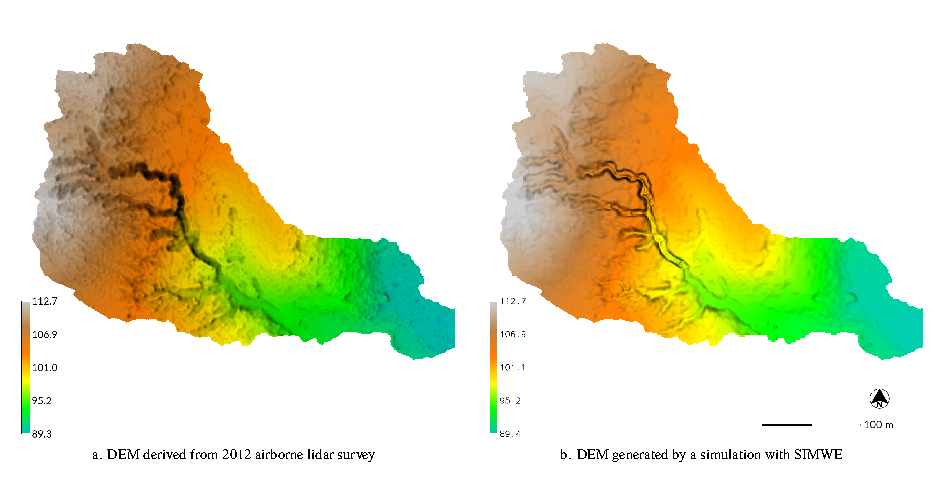
\includegraphics[width=\textwidth,height=0.925\textheight,keepaspectratio]{figures/evolution.pdf}
\caption{
The digital elevation model (DEM) 
before (a) and after (b)
simulated landscape evolution with r.sim.terrain 
for a subwatershed of Patterson Branch, Fort Bragg, NC, USA. 
This simulation used the SIMWE model
for a 120~\unit{min} rainfall event with 25~\unit{mm~hr}$^{-1}$
in a transport limited soil erosion regime at steady state.
In the evolved DEM (b)
the gully channel has widened 
with depositional ridges forming along its thalweg.}
\label{fig:evolution}
\end{figure}

% --------- BODY ---------

\introduction
Landscape evolution models represent how the surface of the earth changes 
over time in response to physical processes. 
Most studies of landscape evolution have been descriptive, 
but a number of numerical landscape evolution models 
have been developed that simulate elevational change over time 
\citep{Temme2013}. 
% numerical models
Numerical landscape evolution models
such as the Channel-Hillslope Integrated Landscape Development (CHILD) model 
\citep{Tucker2001} 
and SIBERIA \citep{Willgoose2005}
simulate steady state flows over long temporal scales. %<-----------------------------ADD LAPSUS
% recent development
\href{http://landlab.github.io/}{Landlab},
a new Python library for numerically modeling Earth surface processes
\citep{Hobley2017},
has components for simulating landscape evolution such as the 
Stream Power with Alluvium Conservation and Entrainment (SPACE) 
model \citep{Shobe2017}.
% gis-based models
While Geographic Information Systems (GIS)
support efficient data management, 
spatial and statistical modeling and analysis, 
and visualization,
there are few GIS-based soil erosion models or landscape evolution models
(see Tables~\ref{table:erosion_models}-\ref{table:evolution_models}).
%%HM ADD HERE r.landscape.evol paper by Isaac or Barton
\cite{Thaxton2004} developed a GRASS GIS shell script module r.terradyn  
to simulate terrain evolution by combining steady-state net erosion deposition rates
estimated by the Simulation of Water Erosion (SIMWE) model \citep{Mitas1998}
and gravitational diffusion. \cite{Barton2010} implemented a long term
landscape evolution GRASS GIS model r.landscape.evol which integrates gravitational diffusion,
USPED model and fluvial erosion and has been applied to simulate impact of prehistoric settlements
on mediteranean landscapes.
% research questions
However, there are still major research questions 
%%HM end changes
to address in the theoretical foundations of erosion modeling 
such as how erosional processes scale over time and space 
and how sediment detachment and transport interact \citep{Mitasova2013}. 
% dynamic evolution
While most numerical landscape evolution models 
simulate peak flows at steady state
(see Table~\ref{table:evolution_models}),
short-term erosional processes like gully formation can be dynamic
with significant morphological changes happening within minutes
before flows reach steady state. 
A landscape evolution model with dynamic water and sediment flow
is needed to study fine-scale spatial and short-term temporal erosional processes
such as gully formation and the development of microtopography. 
%HM should we also say that moels are needed to support sustainable landscape design?
% and study how landscapes can recover from major events?

% steady state versus dynamic
At the beginning of a rainfall event 
the overland water flow regime is dynamic -- 
its depth changes at a variable rate over time and space. 
If the intensity of rainfall continues to change throughout the event
then the flow regime will remain dynamic. 
% steady state
If, however, the overland flow reaches a peak rate
then the hydrologic regime is considered to be at steady state.
At steady state:
% steady state eq.
\begin{equation}
\label{eq:steady_state}
{\partial h(x,y,t) \over \partial t} = 0
\end{equation}
%
{\small
\noindent
where: \\
\noindent
\hspace*{0.5em} $(x,y)$ is the position [\unit{m}]\\
\hspace*{0.5em} $t$ is the time [\unit{s}]\\
\hspace*{0.5em} $h(x,y,t)$ is the depth of overland flow [\unit{m}]\\
}

% gully formation
Gullies are eroded, steep banked channels 
formed by ephemeral, concentrated flows of water.
A gully forms when overland waterflow
converges in a knickzone
-- a concave space with steeper slopes than its surroundings 
\citep{Zahra2017} -- 
during intense rainfall events.  
When the force of the water flow concentrated in the knickzone
is enough to detach and transport large amounts of sediment,
an incision begins to form at the apex of the knickzone 
-- the knickpoint or headwall.
As erosion continues the knickpoint begins to migrate upslope
and the nascent gully channel widens,
forming steep channel banks. 
Multiple incisions initiated by different knickpoints 
may merge into a gully channel
and multiple channels may merge 
into a branching gully system \citep{Mitasova2013}. 
% detachment limited
This erosive process is dynamic; 
the morphological changes drive further changes 
in a positive feedback loop.
When the gully initially forms 
the soil erosion regime should be detachment capacity limited
with the concentrated flow of water in the channel of the gully 
detaching large amounts of sediment 
and transporting it to the foot of the gully, 
potentially forming a depositional fan.
% variable erosion-deposition
If the intensity of rainfall decreases
and transport and detachment capacity 
approach a balance, 
then the soil erosion regime may switch to 
a variable erosion-deposition regime,
in which soil is eroded and deposited 
in a spatially variable pattern.
Subsequent rainfall events may trigger further 
knickpoint formation and upslope migration, 
channel incision and widening, and
depositional fan and ridge formation. 
Between high intensity rainfall events, 
lower intensity events and gravitational diffusion
may gradually smooth the shape of the gully. 
% transport limited
Eventually, if detachment capacity 
significantly exceeds transport capacity
and the regime switches to transport capacity limited, 
the gully may fill with sediment,
as soil continues to be eroded, but is not transported far. 

% gully monitoring
Gully erosion rates and evolution
can be monitored in the field 
or modeled on the computer. 
% field methods
Field methods include
dendrogeomorphology \citep{Malik2008} and 
permanent monitoring stakes for recording erosion rates, 
extensometers for recording mass wasting events, 
weirs for recording water and suspended sediment discharge rates, 
and time series of surveys using 
total station theodolites \citep{Thomas2004},
unmanned aerial systems (UAS),
airborne lidar, and terrestrial lidar \citep{Starek2011,Bechet2016}.
% high resolution topographic data
With terrestrial lidar, airborne lidar and 
UAS photogrammetry
there is now sufficient resolution topographic data 
to morphometrically analyze and 
numerically model fine-scale landscape evolution in GIS
including processes such as gully formation 
and the development of microtopography. 
% gully simulation
Gully erosion has been simulated with 
RUSLE2-Raster (RUSLER)
in conjunction with the Ephemeral Gully Erosion Estimator (EphGEE)
\citep{Dabney2014},
while gully evolution
has been simulated for detachment capacity limited erosion regimes
with the Simulation of Water Erosion (SIMWE) model
\citep{Koco2011, Mitasova2013}. 
Now numerical landscape evolution models 
that can simulate 
steady state and dynamic flow regimes
and can dynamically switch between soil erosion regimes 
are needed to study 
fine-scale spatial and short-term temporal erosional processes.

% aim
The numerical landscape evolution model 
r.sim.terrain was developed to 
simulate the spatiotemporal evolution of landforms
caused by shallow overland water and sediment flows
at spatial scales ranging from
square meters to kilometers
and temporal scales ranging from minutes to years. 
% objectives
This open source, GIS-based landscape evolution model can
simulate either steady state or dynamic flow regimes, 
dynamically switch between soil erosion regimes, and
simulate the evolution of fine-scale morphological features 
such as ephemeral gullies
(Figure~\ref{fig:evolution}).
% questions
It was designed as a research tool for
studying how erosional processes scale over time and space,
comparing empirical and process-based models, 
comparing steady state and dynamic flow regimes, and
studying the role of dynamic flow regimes 
in fine-scale morphological change. 
% testing
r.sim.terrain was tested with 
a subwatershed scale (450~\unit{m}$^{2}$) case study
and the simulations were compared against 
a time-series of airborne lidar surveys.

\section{r.sim.terrain}

% --------- CONCEPT MODEL ---------

%HM sediment flow needs to be replaced by detachment rate for RUSLE
\begin{figure}%[H]
\center
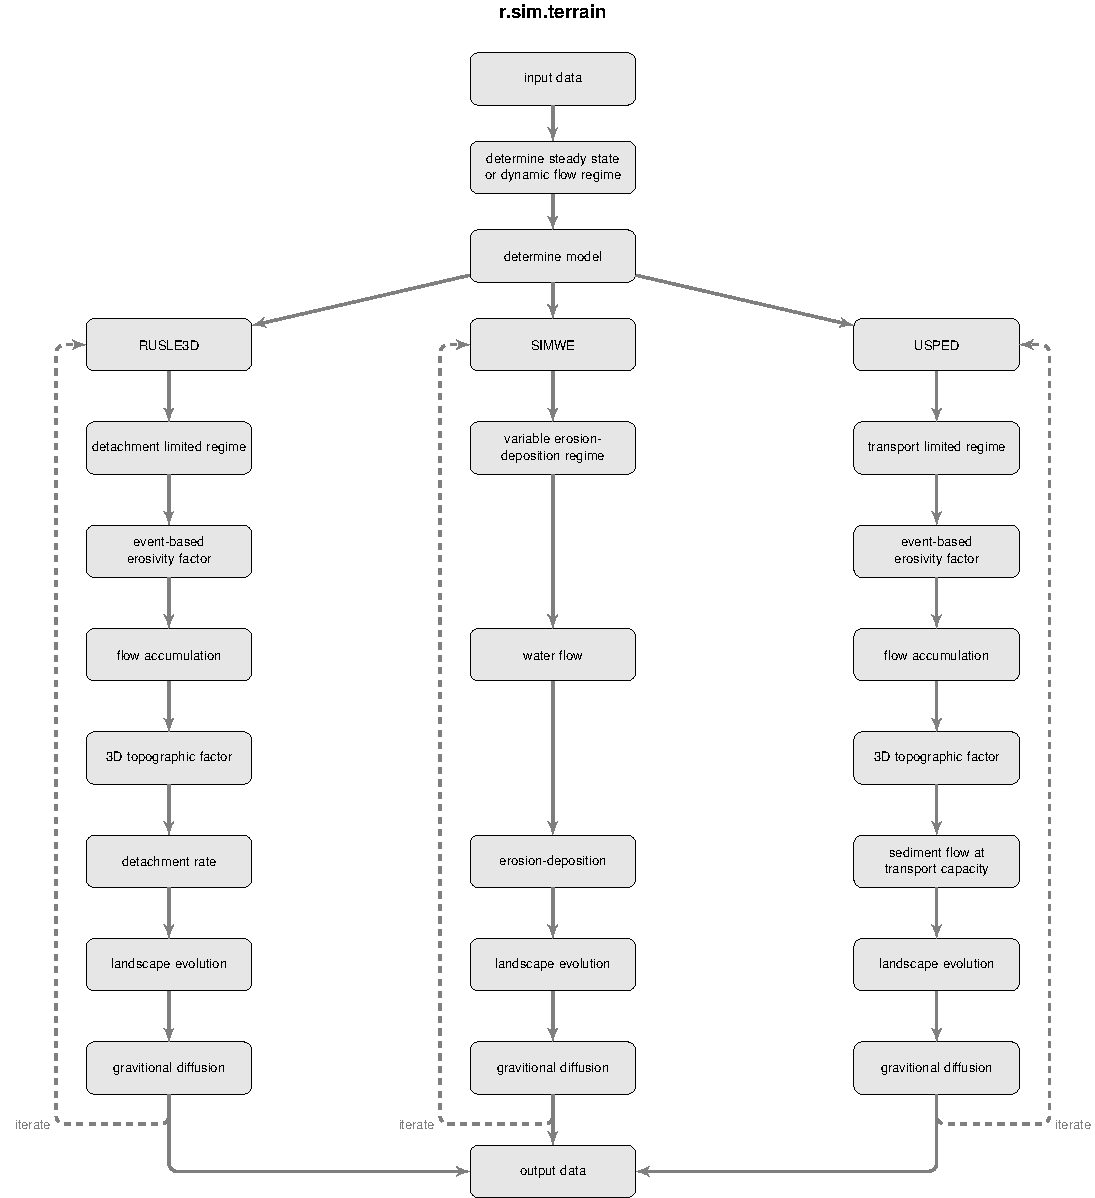
\includegraphics[width=\textwidth,keepaspectratio]{figures/concept.pdf}
\caption{Conceptual diagram for r.sim.terrain. REPLACE SED FLOW BY DETACH IN RUSLE}
\label{fig:evolution}
\end{figure}

% ---------------------------------

The process-based, spatially distributed 
landscape evolution model r.sim.terrain
simulates topographic changes
caused by shallow, overland water flow
across a range of spatiotemporal scales and soil erosion regimes
using either
the Simulated Water Erosion (SIMWE) model, 
the 3-Dimensional Revised Universal Soil Loss Equation (RUSLE 3D) model,
or the Unit Stream Power Erosion Deposition (USPED) model.  
% simwe
SIMWE is a physics-based simulation
that uses a Monte Carlo path sampling method
to solve the water and sediment flow equations 
for detachment limited, transport limited, and variable erosion-deposition 
soil erosion regimes \citep{Mitas1998,Mitasova2004}. 
With SIMWE 
r.sim.terrain
uses the modeled flow of sediment 
-- a function of water flow and soil detachment and transport parameters -- 
to estimate net erosion and deposition rates. 
% rusle3d
%HM fix rusle3d interpretation - this entire section has numerous changes
%HM sediment flows replaced by soil erosion
RUSLE3D is an empirical equation for estimating soil erosion rates
in detachment capacity limited soil erosion regimes \citep{Mitasova1996,Mitasova2013}. 
With RUSLE3D
r.sim.terrain
uses an event-based rainfall erosivity factor, 
the soil erodibility factor, the land cover factor, and the 3D topographic factor (function of slope and the flow accumulation)
to model soil erosion rate.
%HM the 3D topographic factor is function of slope and flow accumulation so mentioning 3D topo factor as a separate factor is confusing
%HM and the soil and cover factors were missing here)
%HM slope, the flow accumulation, and a 3D topographic factor
%HM soil erosion rate is the rate of Soil Loss - that is what RUSLE stands for, not sediment flow
%HMsediment flow. 
% usped
USPED is an semi-empirical equation for net erosion and deposition 
in transport capacity limited soil erosion regimes \citep{Mitasova1996,Mitasova2013}. 
With USPED 
r.sim.terrain
uses an event-based rainfall erosivity factor, 
the soil erodibility factor, the land cover factor, and the 3D topographic factor (function of slope and the flow accumulation)
%HMthe slope and aspect, the flow accumulation, and a 3D topographic factor
to model net erosion or deposition rates as the divergence of sediment flows. 
% evolution
For each of the models topographic change is derived at each time step
from the erosion rate or
%HMsediment flow or 
net erosion-deposition ratei, and gravitational diffusion.
% regimes
%HM water added
The r.sim.terrain model
can simulate either steady state or dynamic water flow regimes.
Depending on the input parameters, simulations with SIMWE 
r.sim.terrain
%HM depending on what we end up using we may use other term than "switch"
can represent variable soil erosion-deposition regimes, including prevailing  
detachment capacity limited, or prevailing transport capacity limited regimes.

% capabilities
The r.sim.terrain model
can simulate the evolution of gullies
including processes such as 
knickpoint migration,
channel incision, 
channel widening, 
aggradation, and
scour pool and 
depositional ridge formation
along the thalweg of the gully. 
% applications
Applications include 
geomorphological research,
erosion control, 
landscape restoration, 
and scenario development 
for landscape planning and management.
% scale
This model can simulate landscape evolution 
over a wide range of spatial scales 
from small watersheds 
less than ten square kilometers
with SIMWE
to regional watersheds
of hundreds of square kilometers
with USPED or RULSE3D,
although it does not model fluvial processes. 
%HM resolutions added - feel free to remove
It has been used at resolutions ranging from sub-meter to 30m.
% implementation
This model has been implemented 
as a Python add-on module 
for the free, open source
\href{https://grass.osgeo.org/}{Geographic Resources Analysis Support System (GRASS) GIS}
\citep{GRASS}. 
The source code is available at 
\url{https://github.com/baharmon/landscape\_evolution} 
under the GNU General Public License v2.
% parallel processing
It supports multithreading and parallel processing
to efficiently compute simulations 
using large, high resolution topographic datasets.
%
The landscape evolution model 
can be installed in GRASS GIS as an add-on module 
with the command: 
\begin{verbatim}
g.extension r.sim.terrain
\end{verbatim}

% -------------- LIMITATIONS ---------------------
%HM why are the limitations here, before we explain what methods are in the model?
%HM is this required this way or can we put them in the discussion after we explain the walkers?
%HM I don't see the metric units as limitation - that is the standard
%HM the real limitation is the lack of fluvial erosion which limits the scale,
%HM lack of full dynamics - we do not have coupled dynamic water and sediment transport and we neglect friction slope
%HM we assume spatially variable but steady rainfal during the modeled landscape evolution time interval
%HM I agree with computational demandsa, although a script can be written to distribute the runs with different seeds
%HM across many processors (we ran it with 50 million particles on computers in 90s). 
Limitations of this landscape evolution model include
shallow overland flow, 
units, computation time, resolution and spatial scale.
% shallow water flow
r.sim.terrain only models shallow overland flows, 
not fluvial processes or subsurface flows. 
% units
It requires data -- including 
elevation and rainfall intensity -- in metric units. 
% computation
%HM the issue of walkers bothers me - we ran it with 50 million walkers on much smaller computers
%HM the algorithm is embarassingly parallel - that means that it can be run on many processors
%HM without any need for comunication - you just start with a different seed
%HM I need to check with Jaro why they have not done the parallelization this way
%HM I think that Anna has added random_seed parameter, so you can run it on many processors 
%Hm starting with a different seed, and then compute the mean sediment flow from all rasters 
%HM and estimate erosion-deposition from that. If time allows we should test this.
The SIMWE model is computationally intensive 
and may require long computation times even with multithreading.
Because SIMWE uses a Green's function Monte Carlo solution 
of the sediment transport equation, 
the accuracy, detail, and smoothness of the results 
depend on the number of random walkers.
While a large number of random walkers will reduce the
numerical error in the path sampling solution,
it will also greatly increase computation time.
Furthermore a customized compilation of GRASS GIS 
is needed for more than 7 million random walkers.
%HM it is not scale but the size of raster that matters 
This limits the size of the raster layers that can be processed
%resolution and spatial scale 
%at which SIMWE can be easily applied,
while RUSLE3D and USPED are much faster, computationally efficient,
and can easily be run for much larger rasters.
%at regional scales. 

% -------------------------- TABLE OF MODELS -----------------------------

% -------------------------- MODEL FIGURE -----------------------------
%HM I modified the caption - I think that you should remove the subcaptions,
%HM editors hate it and most journal formatting does not support it.
%HM make sure you do not refer to 3f as sediment flow - it is erosion rate (see the units)
%HM check the R unit!!!

% model figure
\begin{figure}
\center
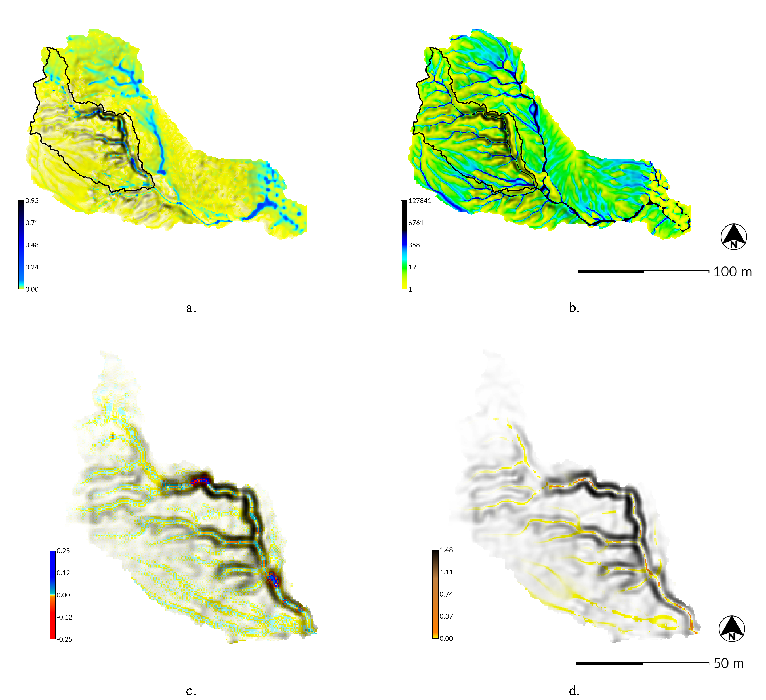
\includegraphics[width=\textwidth,height=0.95\textheight,keepaspectratio]{figures/models.pdf}
\caption{Water flow for a subwatershed (a, d), 
sediment flow and net erosion deposition (b, c)
topographic erosion factor and net erosion (e,f) for
drainage area 1 of Patterson Branch
modeled by SIMWE 
for a 10~\unit{min} event with 50~\unit{mm~hr}$^{-1}$ (a-c)
and by RUSLE3D with a R-factor of 310 UNITS??? 
%~$\unit{MJ~mm~ha^{-1}~hr^{-1}}$ 
(d-f)
}
\label{fig:models}
\end{figure}

% -------------------------- MATH FOUNDATIONS OF THE MODEL -----------------------------

\subsection{Landscape evolution}

Landscape evolution in r.sim.terrain 
is driven by change in elevation surface caused by soil erosion and deposition.
During storm events, overland flow erodes soil, transports sediment across landscape and 
deposits the sediment in some locations. Gravitational diffusion applied to the changed elevation
surface simulates smoothing effects of localized transport of soil between the events.

\subsubsection{Change in elevation} 

% Landscape evolution
Assuming negligible uplift, the change in elevation over time 
${\partial z / \partial t}$ [\unit{m~s}$^{-1}$] 
is described by the continuity of mass equation expressed in terms of divergence 
of sediment flow  \citep{Tucker2001}:
%HM flow or flux above? is flux flow per unit width? check entire paper for consistency
%\citep{Mitasova2013}
% landscape evolution equation
\begin{equation}
\label{eq:evolution} 
{\partial z \over \partial t } = -\nabla~{\bf q_s} = d_s ~ \rho_s^{-1} 
\end{equation}
{\small
where: \\
\noindent
\hspace*{0.5em} $z$ is the elevation [\unit{m}] \\
\hspace*{0.5em} $t$ is the time [\unit{s}] \\
\hspace*{0.5em} ${\bf q_s}$ is the sediment flow per unit width vector [\unit{kg~m}$^{-1}$~\unit{s}$^{-1}$]\\
\hspace*{0.5em} $d_s$ is the net erosion-deposition rate [\unit{kg~m}$^{-2}$~\unit{s}$^{-1}$]\\
\hspace*{0.5em} $\rho_s$ is the sediment mass density [\unit{kg~m}$^{-3}$]\\
}
The overland flow driven net erosion-deposition rate $d_s$ 
 is estimated at different levels of complexity based 
on the user selected simulation mode guided by the type of application.

\noindent
Gravitational diffusion is applied to the changed topography during each time step
to simulate smoothing effects of localized transport of soil that
occurs between rainfall events.
%the settling of sediment particles.
The change in elevation $\partial z / \partial t$
due to gravitational diffusion
is a function of the the sediment mass density,
the diffusion coefficient, and Laplacian of the elevation
%-- i.e.~the sum of the second order derivatives of elevation
\citep{thaxton2004}:
% change in elevation (m) = elevation (m) - (change in time (s) / sediment mass density (kg/m^3) * gravitational diffusion coefficient (m^2/s) * divergence (m^-1))
\begin{equation}
\label{eq:grav_diffusion} 
{\partial z \over \partial t } = \rho_s^{-1} ~ \varepsilon_g ~ \nabla^2 z 
%HM this should be \nabla^2 z, \nabla is an operator so there should be a variable upon which it is applied
%HM see eq 4.41 in Thaxton, also from Willgoose, the second term
\end{equation}
%{\small
\noindent
where $\varepsilon_g$ is the diffusion coefficient [\unit{kg~m}$^{2}$~\unit{s}$^{-1}$].
%\\ \hspace*{0.5em} $\nabla$ is the topographic divergence [\unit{m}$^{-1}$].\\
%}

The discrete implementation follows \citep{Thaxton2004}?:
If it is the same time step we have
\begin{equation}
\label{eq:evolution_disc1} 
z_{t + \Delta t} = z_t + \Delta z_s + \Delta z_g 
\end{equation}
if the time step advances we need two equations, something like this: or see Thaxton
\begin{equation}
\label{eq:evolution_disc1} 
z_{t+ 1/2 \Delta t} = z_t + \Delta z_s  
\end{equation}
\begin{equation}
\label{eq:evolution_disc2} 
z_{t+\Delta t} = z_{t+1/2 \Delta t} + \Delta z_g 
\end{equation}
where $z_{t+ 1/2 \Delta t}'$ is elevation after the change $\Delta z_s$ due to net erosion or deposition (\ref{eq:evolution})
was applied, $z_{t+\Delta t}$ is elevation after the eroded elevation surface
was smoothed by diffusion by adding the diffusion driven elevation change $\Delta z_g$, (\ref{eq:grav_diffusion}).  

\subsubsection{Erosion-deposition regimes}

In general, the net erosion-deposition $d_s$ is obtained by solving the sediment transport continuity equation
which for the simpler, steady state case relates $d_s$ to the divergence 
of sediment flow rate per unit width ${\bf q_s}$ [\unit{kg~m}$^{-1}$~\unit{s}$^{-1}$]:
\begin{equation}
\label{eq:steady_sed}
d_s = \nabla\cdot {\bf q_s} 
\end{equation}
Assuming that the ratio of net erosion-deposition rate $d_s$ to detachment
 capacity  $D_c$  [\unit{kg~m}$^{-2}$~\unit{s}$^{-1}$] 
 plus the ratio of sediment flow rate $q_s = |{\bf q_s}|$ 
to sediment transport capacity $T_c$ [$\unit kg~m^{-1}~s{-1}$] is
 a conserved quantity (unity), as proposed by \cite{fostermeyer72}:
\begin{equation}
\label{eq:foster_law}
d_s/D_c + q_s/T_c = 1
\end{equation}
the net erosion and deposition rates $d_s$ can be expressed as proportional to the difference between
the sediment transport capacity and the actual sediment flow rate \cite{fostermeyer72}:
\begin{equation}
\label{eq:sigma}
d_s =\sigma \bigl[ T_c - q_s\bigr]
\end{equation}
\noindent
where 
%$T_c$ [$\unit kg~m^{-1}~s{-1}$] is the sediment transport capacity,
%$q_s = |{\bf q_s}|$ is the magnitude of sediment flow and 
$\sigma$ [m$^{-1}$] is the first order reaction term
 dependent on soil and cover properties.
The expression for the first order reaction term  is then
\begin{equation}
\label{eq:sigma_Dc_Tc}
\sigma = D_c / T_c
\end{equation}
The qualitative arguments, experimental observations and values for $\sigma$ are discussed, for example, by Foster and Meyer\cite{fostermeyer72} and the concept is used in several well established erosion models such as Water Erosion ... (WEPP) CITE
or RUSLE2???? find the correct name and reference to RUSLE with erdep.

SHOW THE MATH
Using the concept proposed by \cite{fostermeyer72} it is possible to identify two limiting erosion-deposition
regimes.
For $\sigma \to 0$, the net erosion is equal to the detachment capacity
\begin{equation}
\label{eq:detachment_limited}
 d_s = D_c
\end{equation}
For this case, transport capacity of overland flow exceeds
detachment capacity everywhere, erosion and sediment transport is limited by the detachment
capacity and therefore no deposition occurs.
%When rainfall intensity is very high ($i_r \geq 60 \unit{mm~hr}^{-1}$)
An example of this case is a strong storm producing large overland flow over compacted clay soil 
leading to high transport capacity of flow to carry the light clay particles
but low detachment capacity due to compacted soil ($\sigma \leq 0.01 \unit{m}^{-1}$).

For very large $\sigma \to \infty$ the sediment flow is at sediment transport capacity $q_s = T_c$ 
leading to a transport capacity limited regime of erosion-deposition with deposition reaching its maximum
extent for the given water flow. The net erosion-deposition is computed as a divergence of
transport capacity multiplied by a unit vector ${\bf s_0}$ in the direction of flow:
\begin{equation}
\label{eq:transport_limited}
 d_s = \nabla\cdot (T_c . {\bf s_0})
\end{equation}
%This would be the case when rainfall intensity is not very high ($i_r < 60 \unit{mm~hr}^{-1} $) and 
This case may occur, for example, during a moderate storm and overland flow in areas 
with sandy soils with high detachment capacity but
low transport capacity  ($\sigma \geq 100 \unit{m}^{-1}$).

For $0 < \sigma < \infty$ the spatial pattern of net erosion-deposition is variable and depends on the 
relationship between the land cover, soil and topography.
% represented in the governing equations 
%(continuity and Foster's conserved quantity law).
The sediment-transport capacity, $T_c $ and the detachment capacity, $D_c $,
are estimated using water flow shear stress and stream power
expressed as power functions of water-flow properties and slope.    
%For a given rainfall rate and surface roughness, these two variables can be derived from a DEM
%using topographic analysis functions to compute the slope, and flow-routing
%tools to compute the upslope contributing area as an input for estimating unit water flow.
The relation between the parameters of the well known empirical equations for erosion modeling, such as USLE 
and shear stress and stream power was presented by \citep{MooreBurch1984} and used to develop
simple, GIS-based models for the limiting erosion-deposition cases, including RUSLE3D and USPED \citep{Mitasova2001}.
The SIMWE model estimates $T_c$ and $D_c$ using  equations and parameters developed for the WEPP model.

The simulation modes in r.sim.terrain include 
\begin{itemize}
  \item the process-based SIMWE model for steady state and dynamic shallow overland flow 
   and variable erosion-deposition regime with $d_s$ computed 
   by solving the shallow water flow and sediment transport continuity equations,
  \item USPED model for the transport capacity limited regime with $d_s$ computed by equation (\ref{eq:transport_limited})
  \item or RUSLE3D model for the detachment capacity limited case with $d_s$ computed by equation (\ref{eq:detachment_limited}). 
\end{itemize}
The following sections explain the computation of $d_s$ for these three modes in more detail.
%In the detachment capacity limited regime, there is no deposition and $d_s$ represents soil erosion rate (soil loss).

% -------------------------- EROSION-DEPOSITION -----------------------------
\subsection{Simulation of Water Erosion (SIMWE)} \label{simwe}

%THIS ENTIRE SECTION WILL NEED SEVERAL INTERATIONS TO GET IT RIGHT

% simwe intro
SIMWE is a physics-based simulation of shallow overland water and sediment flow
that uses a path sampling method to solve the continuity and momentum equations 
with a 2D diffusive wave approximation 
\citep{Mitas1998,Mitasova2004}.
SIMWE has been implemented in GRASS GIS as the modules 
r.sim.water
and r.sim.sediment. 
% overview
In the SIMWE mode for each landscape evolution time step
r.sim.terrain
computes the first order partial derivatives of elevation surface
$\partial z / \partial x$ and $\partial z / \partial y$, 
%using the GRASS GIS module r.slope.aspect (see the equations in \citep{hofierka2009}),
simulates shallow water flow depth, sediment flow, and net erosion-deposition rate, 
and then evolves the topography based on the erosion-deposition rate
and gravitational diffusion. 
%
The model simulates dynamic flow regimes
when the landscape evolution time step is less than the travel time 
for a drop of water or a particle of sediment to cross the landscape,
e.g. the time step is less than the time to concentration.
With longer landscape evolution time steps the model simulates a steady state regime. 

% <------------------------------------------- EDITS HERE
% "Often, authors presenting a set of governing equations 
% will start with the high-level conservation law(s), 
% and then define each term more precisely. 
% There’s an opportunity to do this at least partly in subsection 2.1.1."
% 
% "So we need a definition for ds, which as suggested above, you could provide in section 2.1.1."
% $q_s$ is the sediment flow rate per unit width [\unit{kg~m}$^{-1}$~\unit{s}$^{-1}$]
% $d_s$ is net erosion-deposition [\unit{kg~m}$^{-2}$~\unit{s}$^{-1}$]
% "Net erosion-deposition $d_s$ -- the difference between sources and sinks --"
% "The basic relationship describing sediment transport by overland flow
% is the sediment continuity equation, 
% which relates the change in sediment storage over time, 
% and the change in sediment flow rate along the
% hillslope to effective sources and sinks 
% (e.g., Haan et al., 1994; Govindaraju and Kavvas, 1991; Foster and Meyer, 1972; Bennet, 1974)."
% ------------------------------------------------------------------------------

%Although the difference between steady-state and dynamic flow regimes is discussed, the differences between the erosion regimes (e.g. detachment capacity limited, transport capacity limited, erosion-deposition and detachment limited) are less clear. A more thorough discussion of those regimes and their differences would allow for a clearer understanding of the results of the model compared to the typical characteristics associated with these regimes. On P16 L24 to L27, the results of SIMWE were compared to the characteristics typical of the simulated erosion regime. Establishing the characteristics of the erosion regimes earlier, perhaps after the explanation of the flow regimes, would give the reader more clarity regarding what influences these regimes and how the model compares to real-world characteristics.

%HM I am re-organizing this, starting with water flow, then sediment continuity equation and erosion regimes will be the last
%HM we may consider moving the descriptive characterization of regimes to the descriptive section of r.sim.terrain 

\subsubsection{Shallow water flow}

%HM we use bold font for vector, feel free to replace it with a symbol with arrow on the top)
% Shallow water flow
The SIMWE model simulates shallow overland water flow
controlled by spatially variable topographic, soil, landcover, 
and rainfall parameters by solving the water flow continuity equation 
%for steady state water flow 
using Green's function Monte Carlo path sampling method 
(Fig.~\ref{fig:models}a). 
In general, shallow water flow ${\bf q}$ is approximated by
the bivariate form of the St.~Venant equation (e.g., \citep{Julien1995}):
% shallow water flow eq.
\begin{equation}
\label{eq:water}
{\partial h \over \partial t} =
 i_e - \nabla ~ {\bf q}
\end{equation}
{\small
\noindent
where: \\
\noindent
%\hspace*{0.5em} $x, y$ is the position [\unit{m}]\\
\hspace*{0.5em} $t$ is the time [\unit{s}] \\
\hspace*{0.5em} $h$ is the depth of overland flow [\unit{m}]\\
\hspace*{0.5em} $i_e$ is the rainfall excess [$\unit{m~s^{-1}}$]
(i.e.~rainfall intensity $-$ infiltration $-$ vegetation intercept)\\
\hspace*{0.5em} $\nabla$ is the divergence operator\\
\hspace*{0.5em} ${\bf q}$ is the vector of water flow per unit width [$\unit{m}^2~\unit{s}^{-1}$]. \\
}

The path sampling method solves the continuity equation by accumulation of the evolving source
over the given time period and this accumulation process can be interpreted as
an approximation of a dynamical solution,
with diffusive wave effects incorporated by adding a diffusion term proprtional to
$ \nabla^2 [h^{5/3}]$
into the solution:
\begin{equation}
\label{eq:difwater}
-{\varepsilon_w\over 2 }\nabla^2 ~ h^{5/3}
+\nabla ~ {\bf q} = i_e
\end{equation}
{\small
\noindent
 where: \\
 \noindent
 \hspace*{0.5em} $\varepsilon_w$ is a spatially variable diffusion coefficient [$\unit{m}^{4/3}~\unit{s}^{-1}$]. \\
}
The solution assumes that water flow velocity is mostly controlled by terrain slope and surface roughness 
and its change during the simulated event at a given location is negligible. 
The water depth $h$ at time $t$ during the simulated rainfall event
%HM note that we have several time steps in r.sim.terrain - topo evolution time step, water flow time step and sediment flow time step
 is computed as function of particle (walkers) density at each grid cell. 
The initial number of particles per grid cell is proportinal to rainfall excess rate $i_e$ (source)
and the particles are then routed across the landscape by finding a new position of the walker at time $\tau + \Delta \tau$ by:
DO WE NEED v0 here? remove 0 if not needed.
\begin{equation}
{\bf r}_m^{new}={\bf r}_m + \Delta \tau {\bf v}_0 + {\bf g}
\end{equation}

{\small
\noindent
where: \\
\noindent
\hspace*{0.5em} ${\bf r} = (x, y)$ is the $m^{th}$ walker position [\unit{m}]\\
\hspace*{0.5em} $\Delta \tau$ is the praticle routing time step [\unit{s}]\\
\hspace*{0.5em} ${\bf g}$ is a random vector with gaussian components with variance $\tau$ ????  [\unit{m}]\\
\hspace*{0.5em} ${\bf v}_0 $ is the velocity vector [$\unit{m~s^{-1}}$],  
 with the direction given by the topographic gradient $\nabla z = (\partial z / \partial x, \partial z / \partial y)$
and magnitude computed by Manning or Chezy equation $v=n^{-1}h^{0.6}S^{0.5}$, where $S$ is slope\\ 
}
%HM should we say here that it is a kinematic wave with diffusion
%HM add here the diagram of dynamic water flow from Lubos here?
The mathematical background of the method is presented in \citep{Mitas1998,Mitasova2005}, including the incoporation
of approximate momentum through increased diffusion rate in the prevailing direction of flow.

% ------------------------------------------------------------------------------

\subsubsection{Sediment flow and net erosion-deposition}

% Sediment flow
In SIMWE the sediment flow over complex topography is approximated 
by the sediment-continuity equation,
which relates the change in sediment storage over time, and the change
in sediment flow rate to effective sources and sinks \citep{haan1994,govindar1991,foster1972}: 

\begin{equation}
\label{eq:sedcont}
{\partial [\rho_s~h] \over \partial t} +
\nabla\cdot {\bf q_s} = {\rm sources - sinks}=
d_s
\end{equation}
\noindent

{\small
\noindent
where: \\
\noindent
\hspace*{0.5em} $\rho_s$ is sediment mass density [$\unit{kg~m^{-3}}$]\\
\hspace*{0.5em} $h$ is water flow depth  [\unit{m}]\\
\hspace*{0.5em} ${\bf q_s}$ is the sediment flow rate per unit width (unit sediment load) vector [$\unit{kg~m^{-1}~s{-1}}$]\\
\hspace*{0.5em} $d_s$ is the net erosion or deposition rate [$\unit{kg~m^{-2}~s^{-1}}$].
}

%DO WE NEED THIS HERE?
%The sediment-flow rate ${\bf q_s}$ is a function of water flow and sediment concentration:
%\citep{Mitas1998}, (Fig.~\ref{fig:models}b):
%\begin{equation}
%\label{eq:sedflow}
%  {\bf q_s} = \rho_s {\bf q}
%\end{equation}
%
%{\small
%\noindent
%where: \\
%\hspace*{0.5em} $\bf q$ is the water flow direction and rate per unit width [$\unit{m^2~s^{-1}}$]\\
%\hspace*{0.5em} $\rho_s$ is sediment mass density in the water column [\unit{kg~m}$^{-3}$].\\
%}

Similarly as for the shallow water flow, SIMWE module solves the sediment flow 
equation using Green's function Monte Carlo path sampling method
assuming that the change in water flow
and sediment concentrations over the modeled time interval at a given location is close to zero.
The sediment flow equation (\ref{eq:ssediment}) 
%which relates the net erosion or deposition
%rate $d_s$ to the divergence of sediment flow rate per unit width ${\bf q_s}$
%
%\begin{equation}
%\label{eq:steady_sed}
%\nabla\cdot {\bf q_s} = d_s 
%\end{equation}
is rewritten to include a small diffusion term proportional to the 
mass of water-carried sediment per unit area $\nabla^2 \varrho$ :
\begin{equation}
\label{eq:difsedim}
-{\varepsilon_s \over 2}\nabla^2 \varrho
+ \nabla\cdot [\varrho {\bf v}]
 + \varrho \sigma |{\bf v}|
= \sigma~T_c = SOURCE (D_c?)
%\sigma({\bf r}) T({\bf r})=Dc/T * T=Dc
\end{equation}
{\small
\noindent
where: \\
\noindent
\hspace*{0.5em} $\varepsilon_s$ is the diffusion constant [$\unit{m^2~s^{-1}}$]\\
\hspace*{0.5em} $\varrho = \rho_s~c~h$ is the mass of sediment transported by water per unit area [$\unit{kg~m^{-2}}$] \\
\hspace*{0.5em} $c$ is the sediment concentration [$\unit{particle~m^{-3}}$].
}

On the left hand side of the equation (\ref{eq:difsedim}), the first term
describes local diffusion, the second term is a drift driven by the water flow
while the third term represents a velocity dependent 'potential' acting on 
the mass of transported sediment. %$\varrho$ EXPLAIN THIS TERM. 
%The equation is solved for $\varrho$ which is represented by particle density.
The initial number of particles per grid cell is proportinal to the soil detachment rate $D_c$
(source) and the particles are then routed across the landscape by finding a new position 
of the walker at time $\tau + \Delta \tau$ by:
\begin{equation}
{\bf r}_m^{new}={\bf r}_m + \Delta \tau {\bf v}_0 + {\bf g}
\end{equation}
 while the updated weight is
\begin{equation}
w_m^{new}=w_m \exp[- \Delta \tau(u({\bf r}_m^{new})+u({\bf r}_m))/2]
\end{equation}
where $u = |{\bf v}_0|????$
The sediment flow is then computed as weighted particle densities 
multiplied by unit vector in the direction of flow
${\bf q_s} = \varrho~{\bf s_0}$ and then net erosion-deposition $d_s$ 
is computed as divergence of sediment flow using equation (\ref{eq:steady_sed}).

SIMWE estimates the detachment capacity sediment-transport capacity, $D_c $, and 
the sediment-transport caacity $T_c $, 
using shear stress and stream power \citep{Mitasova2001}
expressed as power functions of water depth derived by r.sim.water and slope. 

Specifically,  the detachment capacity RESOLVE $\tau$ as time step or shear stress:
\begin{equation}
\label{eq:detach_cap}
D_c =K_d  \bigl(\tau - \tau_0 \bigr)^b = K_d  \bigl(\rho_w\, g h~\sin \beta - \tau_0 \bigr)^b 
\end{equation}
{\small
\noindent
where: \\
\noindent
\hspace*{0.5em} $K_d  [s \; m^{-1}]$ is the effective erodibility (detachment-capacity coefficient) [$\unit{s~m^{-1}}$] for $b=1$ VERIFY\\
\hspace*{0.5em} $\tau$ is the shear stress [$\unit{Pa=kg~m^{-2}}$] \\
\hspace*{0.5em} $\tau_0$ is the critical shear stress [Pa] \\
\hspace*{0.5em} $a$ and $b$ are empirical exponents UNITS? \\
\hspace*{0.5em} CHECK whether we have $\rho_w\, g$ defined already.
}
The shear stress, $\tau $, is a function of water
depth $h$ estimated by r.sim.water and surface slope angle, $\beta [deg] $.

Sediment-transport capacity is computed as:
\smallskip
\begin{equation}
\label{eq:tc_streampower}
T_c =K_s \omega =
K_s n ^{-1} g_w h^{m} (\sin \beta)^{n}, 
\end{equation}
{\small
\noindent
where: \\
\noindent
\hspace*{0.5em} $K_s$ is the effective sediment-transport capacity coefficient [s] \\
\hspace*{0.5em} $m$, $n$ are empirical exponents CHECK both n above - are they the same???
}

% ------------------------------------------------------------------------------
%HM merged into the previous 
%\subsubsection{Erosion-deposition}
%\subsubsection{Erosion regime}
% <---------------------------------------------------EDITING HERE
% REGIMES

%Although the difference between steady-state and dynamic flow regimes is discussed, the differences between the erosion regimes (e.g. detachment capacity limited, transport capacity limited, erosion-deposition and detachment limited) are less clear. A more thorough discussion of those regimes and their differences would allow for a clearer understanding of the results of the model compared to the typical characteristics associated with these regimes. On P16 L24 to L27, the results of SIMWE were compared to the characteristics typical of the simulated erosion regime. Establishing the characteristics of the erosion regimes earlier, perhaps after the explanation of the flow regimes, would give the reader more clarity regarding what influences these regimes and how the model compares to real-world characteristics.

%HM I am re-organizing this, starting with water flow, then sediment continuity equation and erosion regimes will be the last
%HM we may consider moving the descriptive characterization of regimes to the descriptive section of r.sim.terrain 

% Erosion regime
This model can simulate erosion regimes from prevailing detachment limited when XXXXX 
to prevailing transport capacity limited when XXXX and the erosion-deposition patterns in between.
At each landscape evolution time step, the regime can change
based on the rainfall intensity ($i_r$)
and the balance of the sediment detachment capacity ($D_c$),
the sediment transport capacity ($T_c$) and the actual sediment flow rate.
%represented by the first order reaction term $\sigma$,
%which depends on soil and landcover properties.
If the landscape evolution time step is shorter than time to concentration (time for water to reach steady state)
the net erosion-deposition is derived from non-steady state flow...

SUMMARIZE HOW IT IS COMPUTED HERE - refer to discretized equation is we use it
The change in elevation $\Delta z$ is then computed for each time step using the eqation (\ref{eq:evolution})


%HM this was moved to the section 2.1
%When rainfall intensity is very high ($i_r \geq 60 \unit{mm~hr}^{-1}$)
%or $\sigma$ is low, for example, for compacted clay soil with low detachment capacity but 
%high transport capacity ( $\sigma \leq 0.01 \unit{m}^{-1}$),
%then the regime is detachment capacity limited.
%%
%When rainfall intensity is not very high ($i_r < 60 \unit{mm~hr}^{-1} $)
%and $\sigma$ is high, for example, for sandy soils with high detachment capacity but
%low transport capacity  ($\sigma \geq 100 \unit{m}^{-1}$),
%then the regime is transport capacity limited.
%%
%When rainfall intensity is not very high
%($i_r<60 \unit{mm~hr}^{-1}$)
%and $\sigma$ is neither high nor low
%($ 0.01 \unit{m}^{-1}< \sigma < 100 \unit{m}^{-1}$),
%then there is a variable erosion-deposition regime. \\
% erosion regime eq.
%\begin{equation}
%\label{eq:regime}
%\sigma = {D_c \over T_c}
%\end{equation}
%{\small
%\noindent
%where: \\
%\noindent
%%\hspace*{0.5em} $\sigma$  is a first order reaction term [$\unit{m}^{-1}$]\\
%\hspace*{0.5em} $D_c$ is the sediment detachment capacity [$\unit{kg~m}^{-1}s^{-1}$]\\
%\hspace*{0.5em} $T_c$ is the sediment transport capacity [$\unit{kg~m}^{-1}s^{-1}$]\\
%}

% -------------------------------- RUSLE --------------------------------
\subsection{Revised Universal Soil Loss Equation for Complex Terrain (RUSLE3D)}
\label{rusle_model}
RUSLE3D is an empirical model for computing erosion 
in a detachment capacity limited soil erosion regime
for watersheds with complex topography \citep{Mitasova1996}. 
It is based on 
the Universal Soil Loss Equation (USLE),
an empirical equation for estimating the average
sheet and rill soil erosion from rainfall and runoff
on agricultural fields and rangelands with simple topography 
\citep{Wischmeier1978}. 
It models erosion dominated regimes without deposition
in which sediment transport capacity is 
uniformly greater than detachment capacity.
As an empirical equation the predicted soil loss 
is spatially and temporally averaged. 
In USLE soil loss per unit area is determined by 
an erosivity factor $R$,
a soil erodibility factor $K$, 
a slope length factor $L$,
a slope steepness factor $S$,
a cover management factor $C$,
and a prevention measures factor $P$.
These factors are empirical constants derived 
from an extensive collection of measurements 
on 22.13 \unit{m} standard plots with an average slope of 9$\%$.  
RUSLE3D was designed to account for more complex, 3D topography 
with converging and diverging flows. 
In RUSLE3D the topographic potential for erosion at any given point 
is represented by a 3D topographic factor $LS_{3D}$,
which is a function of the upslope contributing area 
and the angle of the slope. 

In this spatially and temporally distributed model 
RUSLE3D is modified by the use of a 
event-based R-factor derived from the rainfall intensity 
at each time step.
For each time step this model computes the parameters for RUSLE3D -- 
an event-based erosivity factor,
the slope of the topography, the flow accumulation, and
the 3D topographic factor -- and then
computes the RUSLE3D equation for soil loss rate (net soil erosion rate). 
The soil erosion rate rate is used to simulate landscape evolution 
in a detachment capacity limited soil erosion regime.

% RESOURCES
% https://ncsu-geoforall-lab.github.io/erosion-modeling-tutorial/erdep_theory.html
% http://www4.ncsu.edu/~hmitaso/gmslab/reports/CerlErosionTutorial/denix/denixstart.html

% ------------------------------------------------------------------------------

\subsubsection{Event-based erosivity factor}

%HM add reference
%HM Citation: Yin, S., M.A. Nearing, P. Borrelli, and X. Xue. 2017. Rainfall erosivity: An overview of methodologies and applications. Vadose Zone J. 16(12).  doi:10.2136/vzj2017.06.0131 - suggests e =0.29[1-0.72exp(-0.082i]
The erosivity factor $R$ 
in USLE and RUSLE 
is the combination of the total energy 
and peak intensity of a rainfall event,
representing the interaction 
between the detachment of sediment particles
and the transport capacity of the flow. 
It can be calculated as the product of the 
the kinetic energy of the rainfall event $E$
and its maximum 30 \unit{min} intensity $I_{30}$
\citep{Brown1987,Renard1997}.
In this model, however, the erosivity factor
is derived at each time step as a function of
kinetic energy, rainfall depth, rainfall intensity, and time.
First rain energy is derived from rainfall intensity \citep{Brown1987}:
VERIFY UNITS FOR ALL EQS BELOW:
%
\begin{equation}
\label{eq:rain_energy}
{e_r = 0.29 ~ [1.-0.72 ~ exp(-0.05 ~ i_r)]}
\end{equation}
%HM
I AM NOT SURE THE GENERALIZED EQ IS BETTER, but it could look like this
\begin{equation}
\label{eq:rain_energy}
{e_r \over e_0} = 1.- b ~ exp(i_r/i_0)
\end{equation}
%
{\small
\noindent
where: \\
\noindent
\hspace*{0.5em} $e_r$is unit rain energy [\unit{MJ~ha}$^{-1}$~\unit{mm}${^-1}$]\\
\hspace*{0.5em} $i_r$ is rainfall intensity [\unit{mm~h}$^{-1}$].\\
\hspace*{0.5em} $b=0.72r$ is coeficient\\
\hspace*{0.5em} $i_0=-1/0.05$ is SEE REVIEWER\\
\hspace*{0.5em} $e_0=0.29$ is SEE REVIEWER
}
The parameters for this equation were derived from observed data and published for different regions by
REFS (US, Greece, others).

%HM I think we have the units here right - show it in the answer
\noindent
Then the event-based erosivity index $R_e$ 
is calculated as the product of 
unit rain energy, rainfall depth, rainfall intensity, and time: 
\begin{equation}
\label{eq:erosivity_index}
{R_e = e_r ~ v_r ~ i_r ~ t_r}
\end{equation}
%
{\small
\noindent
where: \\
\hspace*{0.5em} $R_e$ is the event-based erosivity index [\unit{MJ~mm~ha}$^{-1}$~\unit{hr}$^{-1}$]\\
\hspace*{0.5em} $v_r$ is the rainfall depth [\unit{mm}] derived from ${v_r = i_r~t_r}$\\
\hspace*{0.5em} $t_r$ is the time interval [\unit{s}].
}

% ------------------------------------------------------------------------------

\subsubsection{Flow accumulation}
%
The upslope contributing area per unit width $a$
is determined by flow accumulation (number of grid cells draining into a given grid cell)
 multiplied by grid cell width (Fig.~\ref{fig:models}d). 
Flow accumulation is calculated using 
a multiple flow direction algorithm \citep{Metz2009} 
based on $A^{T}$ least cost path searches \citep{Ehlschlaeger1989}. 
The multiple flow direction algorithm 
implemented in GRASS GIS as the module r.watershed
is computationally efficient, does not require sink filling and can
navigate nested depressions and other obstacles. 

% ------------------------------------------------------------------------------

\subsubsection{3D topographic factor}
%
The 3D topographic factor $LS_{3D}$
is calculated as a function of upslope contributing area
and the slope (Fig.~\ref{fig:models}e). 
\begin{equation}
\label{eq:ls_factor}
LS_{3D} = (m+1) ~ \left({a \over a_0}\right)^m ~ \left({\sin \beta \over \beta_0}\right)^n
\end{equation}
%
{\small
\noindent
where: \\
\noindent
\hspace*{0.5em} $LS_{3D}$ is the dimensionless topographic factor\\
\hspace*{0.5em} $a$ is upslope contributing area per unit width [\unit{m}]\\
\hspace*{0.5em} $a_0$ is the length of the standard USLE plot [22.1 \unit{m}]\\
\hspace*{0.5em} $\beta$ is the angle of the slope [$\degree$]\\
\hspace*{0.5em} $m$ is an empirical coefficient\\
\hspace*{0.5em} $n$ is an empirical coefficient\\
\hspace*{0.5em} $\beta_0$ is the slope of the standard USLE plot [0.09$\degree$]\\
}
The empirical coefficients $m$ and $n$
for the upslope contributing area and the slope
can range from 0.2 to 0.6 and 1.0 to 1.3 respectively
with low values representing dominant sheet flow
and high values representing dominant rill flow.
%
%RESOURCES: http://www4.ncsu.edu/~hmitaso/gmslab/papers/erijgis.html

% ------------------------------------------------------------------------------

\subsubsection{Detachment limited erosion rate}

Erosion rate is a function of the event-based erosivity factor, 
the soil erodibility factor, the 3D topographic factor, cover factor, and the prevention measures factor 
(Fig.~\ref{fig:models}f):
%
\begin{equation}
\label{eq:rusle}
{d_s = E = R_e ~ K ~ LS_{3D} ~ C ~ P}
\end{equation}
%
{\small
\noindent
where: \\
\noindent
\hspace*{0.5em} $E$ is soil erosion rate (soil loss) [\unit{kg~m}$^{-2}$~\unit{min}$^{-1}$]\\
\hspace*{0.5em} $R_e$ is the event-based erosivity factor [\unit{MJ~mm~ha}$^{-1}$~\unit{hr}$^{-1}$]\\
\hspace*{0.5em} $K$ is the soil erodibility factor [\unit{ton~ha~hr~ha}$^{-1}$~\unit{MJ}$^{-1}$~\unit{mm}$^{-1}$]\\
\hspace*{0.5em} $LS_{3D}$ is the dimensionless topographic (length-slope) factor\\
\hspace*{0.5em} $C$ is the dimensionless land cover factor\\
\hspace*{0.5em} $P$ is the dimensionless prevention measures factor.\\
}

% Landscape evolution
\noindent
REFER TO DISCRETE EQUATIONS IF USING
For RUSLE3D the simulated change in elevation 
$\Delta z$
is derived from 
equation \ref{eq:evolution}
for landscape evolution in an detachment limited soil erosion regime
and then equation \ref{eq:grav_diffusion}
for gravitational diffusion.

% -------------------------------- USPED --------------------------------

\subsection{Unit Streampower Erosion Deposition (USPED)} \label{usped_model}
USPED estimates net erosion-deposition as the divergence of sediment flow
in transport capacity limited soil erosion regime.
At transport capacity shallow flows of water are carrying as much sediment as possible 
IF THIS WAS TRUE THERE WOUL BE DEPOSITION EVERWHERE - REMOVE
-- more sediment is being detached 
than can be transported.
WE CAN WRITE: The amount of soil detached is close to the amount of sediment that water flow can cary.
As a transport capacity limited model
USPED predicts erosion where transport capacity increases
and deposition where transport capacity decreases. 
The influence of topography on sediment flow  
is represented by a topographic sediment transport factor,
while the influence of soil and landcover are represented by 
factors adopted from USLE and RUSLE
\citep{Mitasova1996}.
%
The sediment flow is estimated by computing
the event-based erosivity factor ($R_e$) 
using Eq.~\ref{eq:erosivity_index},
the slope and aspect of the topography,
the flow accumulation with a multiple flow direction algorithm,
the topographic sediment transport factor,
and the sediment flow at transport capacity.
The net erosion-deposition is then computed as the divergence of the sediment flow. 

% Topographic sediment transport factor
The 3D topographic factor (Eq.~\ref{eq:ls_factor}) 
for RUSLE3D is adapted to represent 
the topographic sediment transport factor ($LS_T$) --
the topographic component 
of overland flow at sediment transport capacity (REFER HERE TO STREAM POWER - that where USPED name is coming from):
%
\begin{equation}
\label{eq:lst_factor}
{LS_T = a^{m} ~ (\sin \beta)^{n}}
\end{equation}
%
{\small
\noindent
where: \\
\noindent
\hspace*{0.5em} $LS_T$ is the topographic sediment transport factor\\
\hspace*{0.5em} $a$ is the upslope contributing area per unit width [m]\\
\hspace*{0.5em} $\beta$ is the angle of the slope [$\degree$]\\
\hspace*{0.5em} $m$ is an empirical coefficient\\
\hspace*{0.5em} $n$ is an empirical coefficient.\\
}

% Sediment flow at transport capacity
\noindent
The sediment flow at transport capacity is a function of 
the event-based rainfall factor, the soil erodibility factor, 
the topographic component of overland flow,
the landcover factor, and the prevention measures factor:
%
\begin{equation}
\label{eq:usped}
{T = R_e ~ K ~ C ~ P ~ LS_T}
\end{equation}
{\small
\noindent
where: \\
\noindent
\hspace*{0.5em} $T$ is sediment flow at transport capacity [\unit{kg~m}$^{-1}$~\unit{s}$^{-1}$]\\ 
\hspace*{0.5em} $R_e$ is the event-based rainfall factor [\unit{MJ~mm~ha}$^{-1}$~\unit{hr}$^{-1}$]\\
\hspace*{0.5em} $K$ is the soil erodibility factor [\unit{ton~ha~hr~ha}$^{-1}$~\unit{MJ}$^{-1}$~\unit{mm}$^{-1}$]\\ 
\hspace*{0.5em} $C$ is the dimensionless land cover factor\\
\hspace*{0.5em} $P$ is the dimensionless prevention measures factor.\\
}

%Erosion-deposition at transport capacity
\noindent
Net erosion-deposition at transport capacity is estimated as the divergence of sediment flow: 
%D = ∇ · (T s0) = ∂(T cos α)/∂x + ∂(T sin α)/∂y
\begin{equation}\label{eq:usped_erdep} 
d_s = 
{\partial (T ~ \cos \alpha) \over \partial x} +
{\partial (T ~ \sin \alpha) \over \partial y}
\end{equation}
{\small
\noindent
where: \\
\hspace*{0.5em} $d_s$ is net erosion-deposition [\unit{kg~m}$^{-2}$~\unit{s}$^{-1}$]\\
\hspace*{0.5em} $\alpha$ is the aspect of the topography (direction of flow) [$\degree$].\\
}

%Landscape evolution
\noindent
REFER TO DISCRETE EQUATION ID USED
With USPED the simulated change in elevation $\Delta z$
is derived from equation \ref{eq:evolution} for landscape evolution
and then equation \ref{eq:grav_diffusion}
for the gravitational diffusion.

% -------------------------------- CASE STUDIES --------------------------------

\section{Case study} 

Military activity is a high-impact land use 
that can cause significant physical alteration to the landscape. 
Erosion is a major concern for military installations, 
particularly at training bases, 
where the land surface is disturbed by 
off-road vehicles, foot traffic, and munitions. 
Off-road vehicles and foot traffic by soldiers 
cause the loss of vegetative cover, 
the disruption of soil structure, soil compaction, 
and increased runoff due to 
reduced soil capacity for water infiltration 
\citep{Webb1983, McDonald2004}.
Gullies -- ephemeral channels with steep headwalls 
that incise into unconsolidated soil to depths of meters -- 
are a manifestation of erosion common to 
military training installations like Ft. Bragg in North Carolina 
and the Piñon Canyon Maneuver Site in Colorado. 
While the local development of gullies can restrict 
the maneuverability of troops and vehicles during training exercises, 
pervasive gullying across a landscape 
can degrade an entire training area 
\citep{Huang2014}.

To test the effectiveness of the different models 
in r.sim.terrain
we compared the simulated evolution
of a highly eroded subwatershed of 
Patterson Branch on Fort Bragg, North Carolina
against a timeseries of airborne lidar surveys.
The models -- SIMWE, RUSLE3D, and USPED --
were tested in steady state and dynamic modes
for constant rainfall, design storms, and recorded rainfall.

\subsection{Patterson Branch}

\begin{figure}
\center
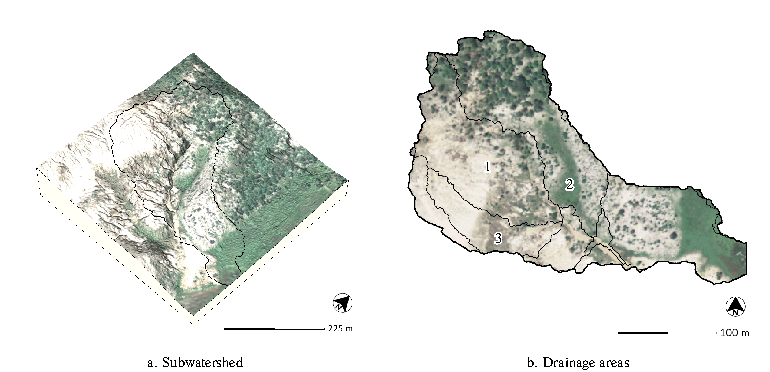
\includegraphics[width=\textwidth,height=0.95\textheight,keepaspectratio]{figures/watershed.pdf}
\caption{Subwatershed with 2014 orthoimagery
draped over the 2016 digital elevation model (a)
and drainage areas with 2014 orthoimagery (b), Patterson Branch, Fort Bragg, NC, USA}
\label{fig:watershed}
\end{figure}

With 650~\unit{km}$^{2}$ of land
Fort Bragg is the largest military installation in the US
and has extensive areas of bare, erodible soils
on impact areas, firing ranges, landing zones, and dropzones. 
It is located in the Sandhills region of North Carolina 
with a Longleaf Pine and Wiregrass Ecosystem \citep{Sorrie2006}.
%
The study landscape 
-- a subwatershed of Patterson Branch (Figure~\ref{fig:watershed}a) 
in the Coleman Impact Area --
is pitted with impact craters from artillery and mortar shells
and has an active, approximately 2~\unit{m} deep gully. 
%
It is a Pine-Scrub Oak Sandhill community
composed primarily of Longleaf Pine (\emph{Pinus palustris})
and Wiregrass (\emph{Aristida stricta})
on Blaney and Gilead loamy sands 
\citep{Sorrie2004}. 
%
Throughout the Coleman Impact Area
frequent fires ignited by live munitions
drive the ecological disturbance regime
of this fire adapted ecosystem.
%
In 2016 the  450~\unit{m}$^{2}$ study site was
43.24\% bare ground with predominately loamy sands,
39.54\% covered by the Wiregrass community, and
17.22\% forested with the Longleaf Pine community 
(Figure~\ref{fig:study_area}a). 
%
We hypothesize that the elimination of forest cover
in the impact zone
triggered extensive channelized overland flow,
gully formation, and sediment transport into the creek. 

% --------- DATA ---------
Timeseries of digital elevations models 
and landcover maps for the study landscape
were generated from lidar pointclouds and orthophotography.
%(Figure~\ref{fig:study_area}a-c). 
The digital elevations models for 2004, 2012, and 2016
were interpolated at 0.3~\unit{m} resolution
using the regularized spline with tension function \citep{Mitasova1993,Mitasova2005}
from airborne lidar surveys 
collected by the NC Floodplain Mapping program and Fort Bragg. 
%
Unsupervised image classification 
was used to identify clusters of spectral reflectance
in a timeseries of 1~\unit{m} resolution orthoimagery 
collected by the National Agriculture Imagery Program.
The landcover maps were derived from the
classified lidar point clouds and the classified orthoimagery.
Spatially variable soil erosion factors 
-- k-factor, c-factor, mannings, and runoff rates --
were then derived from the landcover and soil maps.
The dataset for this study is hosted at 
\url{https://github.com/baharmon/landscape\_evolution_dataset}
under the ODC Open Database License (ODbL).
The data is derived from publicly available data from
the US Army, USGS, USDA, Wake County GIS, NC Floodplain
Mapping Program, and the NC State Climate Office.
There are detailed instructions for preparing the input data in the 
\href{https://github.com/baharmon/landscape_evolution/blob/master/tutorial.md}{tutorial}
and a complete record of the commands used to process the sample data in the
\href{https://github.com/baharmon/landscape_evolution_dataset/blob/master/nc_spm_evolution/DATA.md}{data log}.

% --------- MORPHOLGY ---------
We used the geomorphons method 
of automated landform classification
based on the openness of terrain \citep{Jasiewicz2013}
and the difference between the digital elevation models 
to analyze the changing morphology of the study area
(Figure~\ref{fig:study_area}c-d). 
%
The 2~\unit{m} deep gully -- 
its channels classified as valleys and 
its scour pits as depressions by geomorphons -- 
has multiple mature branches
and ends with a depositional fan.
%
The gully has also developed 
depositional ridges beside the channels.
Deep scour pits have developed 
where branches join the main channel 
and where the main channel has sharp bends.
%
A new branch has begun to form 
in a knickzone classified as a mix of valleys and hollows
on a grassy swale on the northeast side of the gully.
Between 2012 and 2016 a depositional ridge
has developed at the foot of this nascent branch
where it would meet the main channel. 
%
The difference in elevation between 2012 and 2016
(Figure~\ref{fig:study_area}b)
shows a deepening of the main channel 
by approximately 0.2~\unit{m} 
and the scours pits
by approximately 1~\unit{m},
while depositional ridges have formed and grown up to
approximately 1~\unit{m} or more.

% study area figure
\begin{figure}
\center
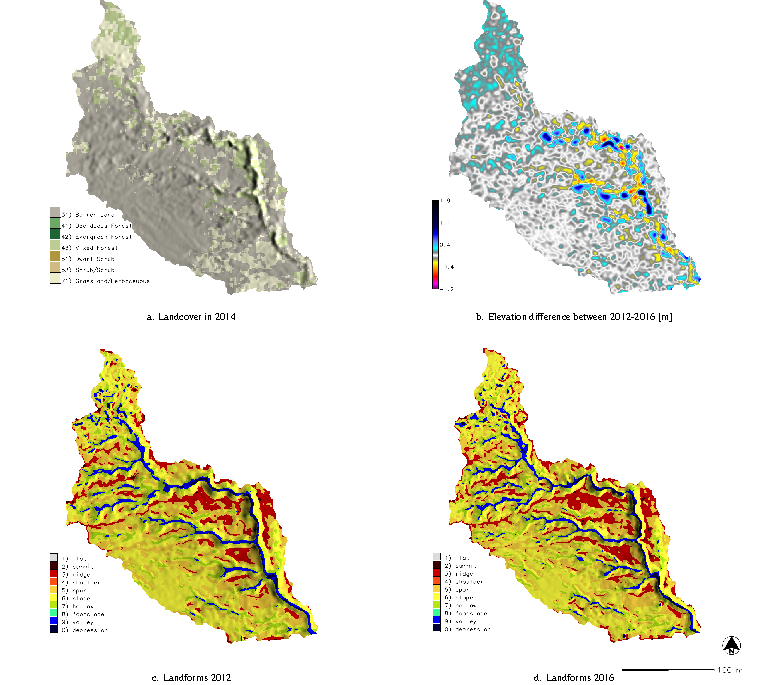
\includegraphics[width=\textwidth,height=0.95\textheight,keepaspectratio]{figures/study_area.pdf}
\caption{Morphological Change, Drainage Area 1, Study Subwatershed, Patterson Branch, Fort Bragg, NC, USA}
\label{fig:study_area}
\end{figure}

% --------- SIMULATIONS ---------
\subsection{Simulations}
%
We ran a sequence of r.sim.terrain simulations 
with design storms
for the Patterson Branch subwatershed study area
to test and demonstrate the capabilities 
of the RUSLE3D, USPED, and SIMWE models
(Table~\ref{table:simulations}).
%
Since the study area was dominated by
a variable erosion-deposition or transport limited
soil erosion regime during the 2012-2016 study period, 
we could not quantitatively assess 
the detachment capacity limited models
against the observed topographic evolution of the landscape.
%
Instead the goal of simulations was to test
what morphological processes and features 
the different models could simulate. 
%
We analyzed the results of the simulations 
by qualitatively comparing landforms 
and the net difference in elevation
and by quantitatively comparing 
linear regressions of elevation change.

% design storms
While r.sim.terrain can use rainfall records,
we used design storms to demonstrate and test 
the basic capabilities of the model. 
Our design storms are based off the peak rainfall values
in records from the State Climate Office of North Carolina.
% parameters
We used RUSLE3D to simulate landscape evolution
in a dynamic, detachment capacity limited soil erosion regime
for a 120~\unit{min} design storm
with 3~\unit{min} intervals 
and a constant rainfall intensity of 50~\unit{mm~hr}$^{-1}$
(Figure~\ref{fig:simulations}a-b).
%
We used USPED to simulate landscape evolution
in a dynamic, transport capacity limited soil erosion regime
for a 120~\unit{min} design storm
with 3~\unit{min} intervals 
and a constant rainfall intensity of 50~\unit{mm~hr}$^{-1}$
(Figure~\ref{fig:simulations}c-d).
%
We used SIMWE to simulate landscape evolution
in a steady state, variable erosion-deposition soil erosion regime
for a 120~\unit{min} design storm
with a constant rainfall intensity of 50~\unit{mm~hr}$^{-1}$
(Figure~\ref{fig:simwe_simulations}a-b). 
%
We also used SIMWE to simulate landscape evolution
in a steady state, detachment capacity limited soil erosion regime
for a 120~\unit{min} design storm
with a constant rainfall intensity of 25~\unit{mm~hr}$^{-1}$
(Figure~\ref{fig:simwe_simulations}c-d).
We used a lower rainfall intensity for this simulation 
to reduce overshoot.
%
In all of the simulations 
a sink filling algorithm
-- an optional parameter in r.sim.terrain -- 
was used to reduce the effects of positive feedback loops
that cause the over-development of scour pits. 

% scripts
The simulations were automated and run in parallel
using Python scripts that are available in the 
\href{https://github.com/baharmon/landscape_evolution}{software repository}.
% reproducibility
The simulations can be reproduced using these scripts
and the study area dataset 
by following the instructions 
in the Open Science Framework repository 
at \url{https://osf.io/tf6yb/}.
% benchmarks
The simulations were run 
in GRASS GIS 7.4 
on a desktop computer 
with 64-bit Ubuntu 16.04.4 LTS,
8 x 4.20 GHz Intel Core i7 7700K CPUs,
and 32 GB RAM. 
% multithreading
Simulations using SIMWE 
are far more computationally intensive
than RULSE3D or USPED, 
but support multi-threading 
when compiled with OpenMP. 
% runtime
Dynamic simulations of RUSLE3D and USPED each took
3~\unit{min}~14~\unit{s} to run on a single thread, 
while steady state simulations for SIMWE each took 
84~\unit{min}~13~\unit{s} running on 6 threads
(Table~\ref{table:simulations}).


% --------- RESULTS ---------
\subsection{Results}

% linear regression
We used linear regression to quantitatively analyze 
observed versus simulated changes in topographic elevation
(Table~\ref{table:linear_regression}).
As expected given that the gully was dominated 
by a variable erosion-deposition 
or  transport capacity limited soil erosion regime 
throughout the study period,
the detachment capacity limited models 
diverged more from the 2012-2016 baseline. 

% dynamic model results
The dynamic RUSLE3D simulation
deepened the main channel of the gully,
while the dynamic USPED simulation
eroded the banks of the gully
and deposited in channels
causing the gully grow wider and shallower
(Figure~\ref{fig:simulations}). 
%
As a detachment capacity limited model
RUSLE3D's results were
dominated by erosion and 
thus negative elevation change.
%
RUSLE3D carved a deep incision 
in the main gully channel
where water and sediment flow accumulated
(Figure~\ref{fig:simulations}c). 
%
As a transport capacity limited model
USPED generated a distributed pattern
with both erosion and deposition and thus
negative and positive elevation change. 
%
While USPED's pattern of elevation change
was grainy and fragmented, 
it captured the process of channel 
filling and widening expected with 
a transport capacity limited soil erosion regime
(Figure~\ref{fig:simulations}f). 

% steady state model results
The steady state SIMWE simulations 
predicted more realistic morphological patterns 
of landscape evolution
(Figure~\ref{fig:simwe_simulations}). 
%
For transport limited and
variable erosion-deposition regimes
SIMWE simulated
channel widening 
and the formation of depositional ridges
along the thalweg of the channel
(Figure~\ref{fig:simwe_simulations}c).
%
For a detachment limited soil erosion regime
SIMWE simulated major erosion
driving the continued development 
of the gully network
including the spread of rills and
the evolution of the nascent branch
into a full fledged channel
(Figure~\ref{fig:simwe_simulations}f). 
%
The detachment limited simulation
also formed extensive ridges
beside the gully channels 
(Figure~\ref{fig:simwe_simulations}f), 
continuing the development of 
channel-side ridges
observed in the 2012 and 2016 landform maps
(Figure~\ref{fig:study_area}e-f). 

% comparison of dynamic and steady state results
Given the presence the mature gully 
with ridges along its banks,
this landscape had previously been dominated by 
a detachment limited soil erosion regime.
%
The detachment limited SIMWE simulation 
generated the morphological features
-- the deeply incised gully channels, 
scour pits,
and ridges along the channels 
--
characteristic of a detachment-limited erosion regime,
realistically simulating landscape evolution 
at the scale of a subwatershed. 
%
The erosion-deposition and transport limited 
SIMWE simulations also generated 
the morphological processes and features
that would be expected in these regimes
-- gradual aggradation
and the formation of a depositional ridge 
along the thalweg of the channel.

While RUSLE3D and USPED
produced less realistic patterns of landscape evolution
than SIMWE,
these models were much faster and still generated
the key morphological patterns and processes -- 
channel incision, filling, and widening. 
%
Given their speed
and approximate modeling of erosive processes, 
RUSLE3D and USPED 
are effective for simulating landscape evolution
at regional scales, 
i.e.~for landscapes greater than 10~\unit{km}$^{2}$. 
%
RUSLE3D for example has been used to
model erosion for the entire 650~\unit{km}$^{2}$ 
Fort Bragg installation at 9~\unit{m} resolution
\citep{Levine2018}. 

% --------- SIMULATION TABLES ---------

% linear regression table

% --------- SIMULATION FIGURES ---------

% dynamic figure
\begin{figure}
\center
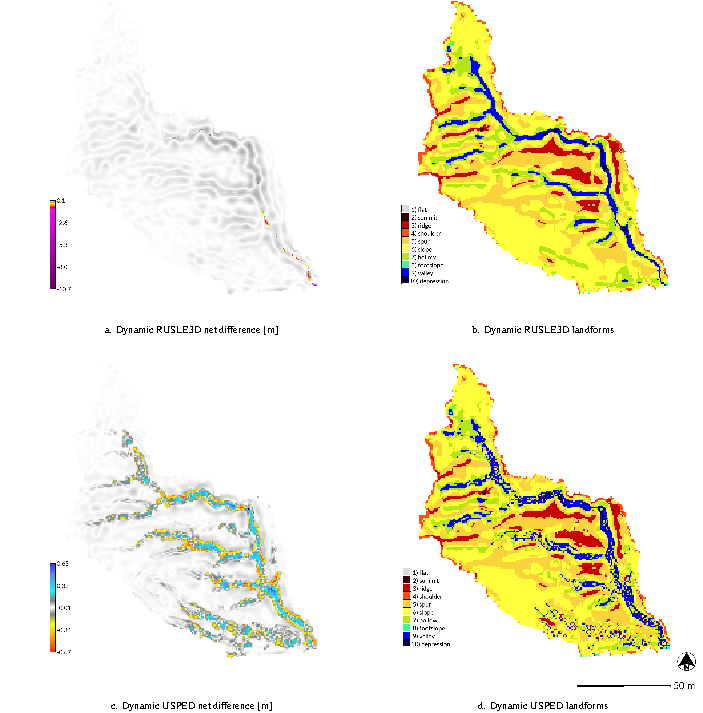
\includegraphics[width=\textwidth,height=0.925\textheight,keepaspectratio]{figures/simulations.pdf}
\caption{Dynamic RUSLE3D (a-b) and USPED (c-d) simulations
for a 120~\unit{min} event with a rainfall intensity of 50~\unit{mm~hr}$^{-1}$,\\
Drainage Area 1, Study Subwatershed, Patterson Branch, Fort Bragg, NC}
\label{fig:simulations}
\end{figure}

% steady state simwe figure
\begin{figure}
\center
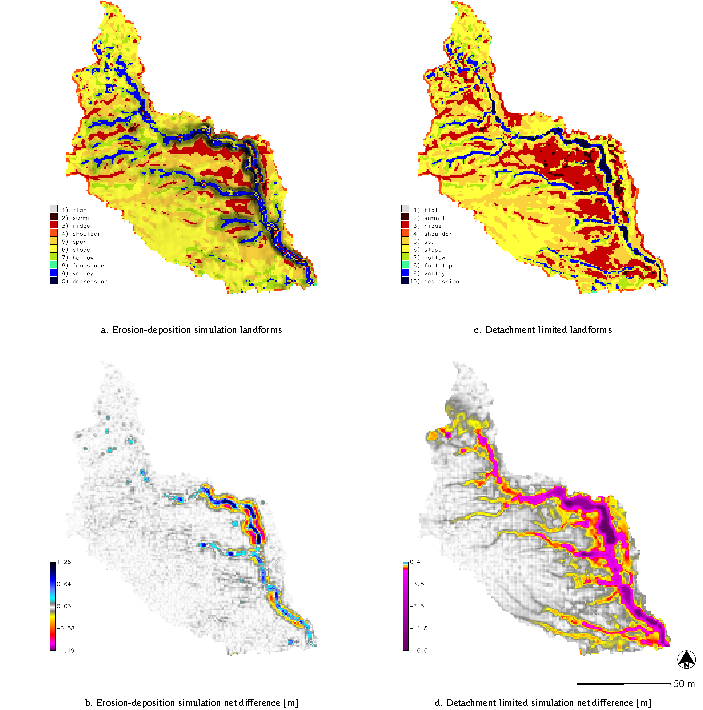
\includegraphics[width=\textwidth,height=0.95\textheight,keepaspectratio]{figures/simwe.pdf}
\caption{Steady state SIMWE simulations
for 120~\unit{min} events with rainfall intensities of 50~\unit{mm~hr}$^{-1}$ (a-b)
and 25~\unit{mm~hr}$^{-1}$ (c-d),\\
Drainage Area 1, Study Subwatershed, Patterson Branch, Fort Bragg, NC}
\label{fig:simwe_simulations}
\end{figure}

% -------------------- CONCLUSIONS ---------------------------------
\conclusions

The short-term landscape evolution model 
r.sim.terrain 
can realistically simulate the development of 
gullies, rills, and hillslopes by overland water erosion
for a range of hydrologic and soil erosion regimes.
The landscape evolution model was tested
with a series of simulations for different 
hydrologic and soil erosion regimes
for a highly eroded sub-watershed on Fort Bragg
with an active gully.
For each regime it generated the 
morphological processes and features expected.
% physics based models
The physics-based SIMWE model 
realistically simulated short-term topographic change
for steady state hydrologic regimes
at sub-watershed to watershed scales. 
For detachment limited soil erosion regimes
it simulated morphological processes including
channel incision, channel widening, and 
the development of knickzones, rills, and scour pits.
For transport limited and variable erosion-deposition regimes,
it simulated processes such as channel aggradation,
scouring, and the development of
depositional ridges along the thalweg.
% empirical models
The empirical RUSLE3D and USPED models
approximated short-term topographic change
at watershed to regional scales. 
For detachment limited soil erosion regimes 
RUSLE3D simulated channel incision,
while for transport limited regimes
USPED simulated channel widening and filling. 
% uses & implications
Since it is a GIS-based model 
that realistically simulates 
fine-scale morphological processes and features,
r.sim.terrain can easily and effectively be used 
in conjunction with other GIS-based tools
for geomorphological research,
land management and conservation,
erosion control, and landscape restoration. 

% --------- FUTURE WORK ---------

% assessment study
In the future we plan to assess this model
by comparing simulations against 
a monthly timeseries
of submeter resolution surveys
by unmanned aerial systems and terrestrial lidar. 
% case study
We also plan to develop a case study demonstrating
how the model can be used as a planning tool 
for landscape restoration. 
% enhancements
Planned enhancements to model include 
modeling subsurface flows, 
accounting for bedrock, 
and a reverse landscape evolution mode
for backward modeling. 

% --------------------CODE AND DATA------------------------

\codedataavailability{
% open science
As a work of open science
this study is reproducible, repeatable, and recomputable.
Since the data, model, GIS, dependencies are all 
free and open source, the study can easily be reproduced.
% code
The landscape evolution model 
has been implemented in Python as module
for GRASS GIS, a free and open source GIS.
 The source code for the model is hosted on GitHub at 
\url{https://github.com/baharmon/landscape_evolution}
under the GNU General Public License version 2.
The code repository also includes Python scripts 
for running and reproducing the simulations in this paper. 
The digital object identifier (DOI) 
for the version of the software documented in this paper is:
\url{https://doi.org/10.5281/zenodo.2542921}.
There are detailed instructions for running this model in the manual at
\url{https://grass.osgeo.org/grass76/manuals/addons/r.sim.terrain.html}
and the tutorial at
\url{https://github.com/baharmon/landscape_evolution/blob/master/tutorial.md}.
% data
The geospatial dataset for the study area is available on GitHub at
\url{https://github.com/baharmon/landscape_evolution_dataset}
under the 
\href{https://opendatacommons.org/licenses/odbl/}{Open Database License} 
with the DOI:
\url{https://doi.org/10.5281/zenodo.2542929}.
The
\href{https://github.com/baharmon/landscape_evolution_dataset/blob/master/nc_spm_evolution/DATA.md}{data log} has a complete record of the commands used to process the sample data.
% osf
The source code, scripts, data, and results are also hosted
on the Open Science Framework at 
\url{https://osf.io/tf6yb/}
with the DOI:
\url{https://doi.org/10.17605/osf.io/tf6yb}.
}




% ----------------------------------------------------------------------------

\noappendix 

\authorcontribution{
Brendan Harmon developed 
the models, code, data, case studies, and manuscript.
Helena Mitasova contributed to the development 
of the models and case studies and revised the manuscript.
Anna Petrasova and Vaclav Petras
contributed to the development of the code.
All authors read and approved the final manuscript.
}

\competinginterests{The authors declare that they have no conflict of interest.} 

\begin{acknowledgements}
We acknowledge the GRASS GIS Development Community
for developing and maintaining GRASS GIS.
\end{acknowledgements}

% ---------------------REFERENCES---------------------------
\bibliographystyle{copernicus}
\bibliography{landscape_evolution.bib}

\end{document}
